\section{Task Analysis}
\label{sec:task}
Identify the analysis goals and distill the corresponding visualization tasks is the first yet significant step in designing a useful tool. In this section, we examine how domain experts approach the challenge of analyzing a new model and assess its strength and weakness.
Then, we reify the observations into a common paradigm and identify where and how a visualization tool could help experts interpret the model and development intuitive, more importantly, how the proposed fit into the domain experts' though process and workflow.

During our long-term collaboration with two domain experts in NLP, we have conducted extensive interview and discussion on the common approach researchers employ to interpret the behavior and obtain intuition for a new model.
%
Often, the most important metric for evaluating a model is the prediction accuracy. However, most researchers would agree, the accuracy alone does not provide the full picture. The model could perform much worse on a different test set. The model may produce many correct predictions for the ``wrong'' reasons (e.g., pickup unintended pattern in the training data that does not exist in real word scenarios).
%
As a result, NLP researchers often employ a set of tests, which are driven by their domain knowledge and hypotheses based on the architecture, to assess the model.
%
A stereotypical scenario can be summarized as the follow.
%
To assess a model for a specific NLP task, the research start the analysis by looking at the failure cases.


\shusen{What is the paradigm?}
Look at example, perturb the example, see how the perturb the one fails,

learn the limitation and strength from the where and how the errors occurs. iterate 


\begin{figure}[htbp]
\centering
\vspace{-2mm}
 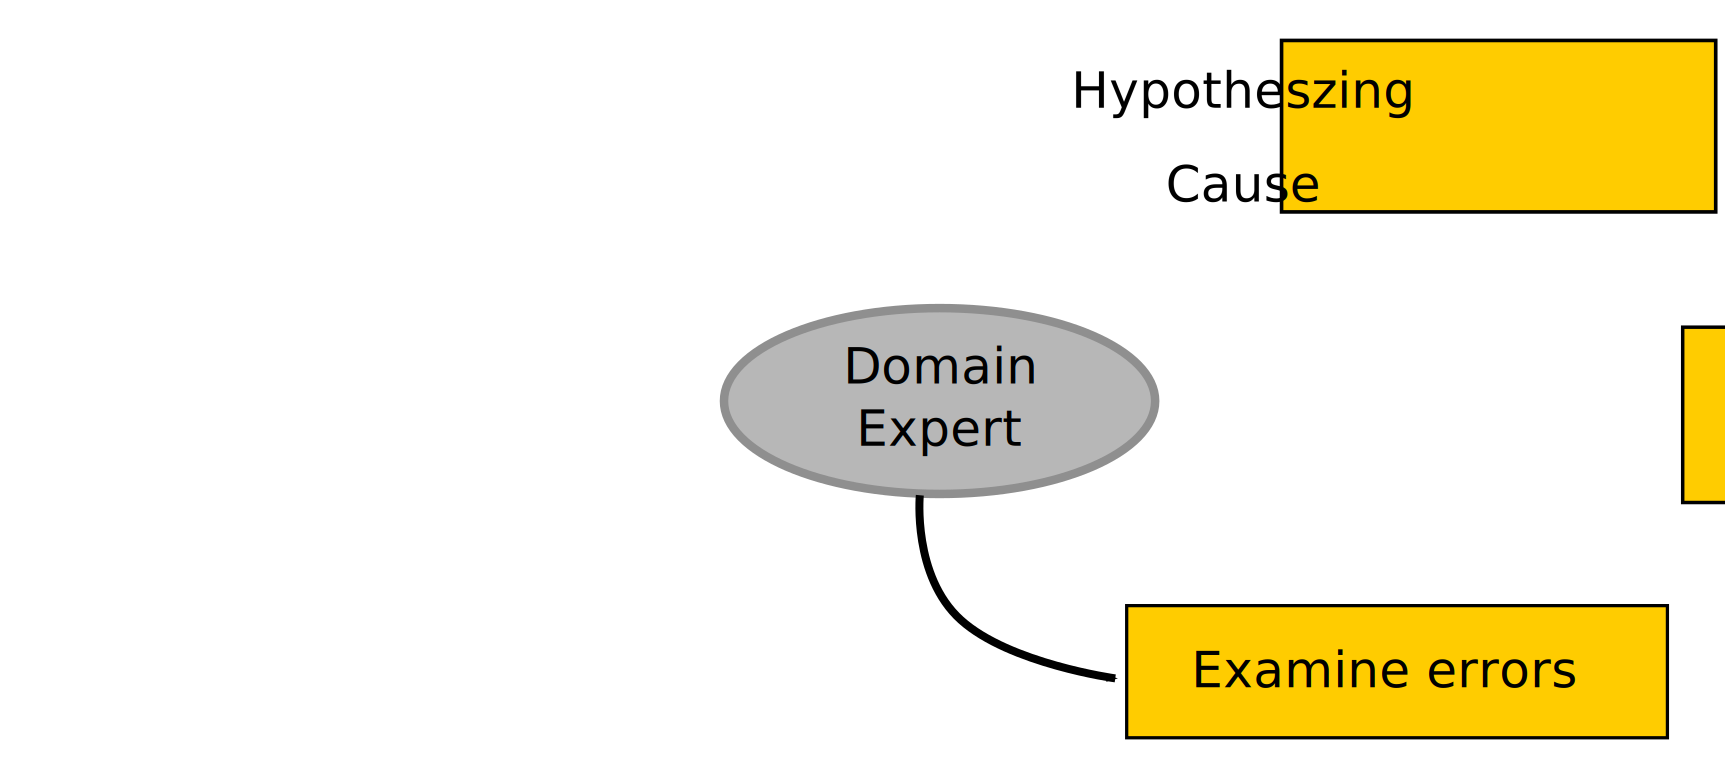
\includegraphics[width=1.0\linewidth]{errorAnalysis}
 \caption{How domain experts carry out error analysis on the model.}
\label{fig:modelPipeline}
\end{figure}

In this section,
